% Options for packages loaded elsewhere
\PassOptionsToPackage{unicode}{hyperref}
\PassOptionsToPackage{hyphens}{url}
%
\documentclass[
]{article}
\usepackage{amsmath,amssymb}
\usepackage{lmodern}
\usepackage{iftex}
\ifPDFTeX
  \usepackage[T1]{fontenc}
  \usepackage[utf8]{inputenc}
  \usepackage{textcomp} % provide euro and other symbols
\else % if luatex or xetex
  \usepackage{unicode-math}
  \defaultfontfeatures{Scale=MatchLowercase}
  \defaultfontfeatures[\rmfamily]{Ligatures=TeX,Scale=1}
\fi
% Use upquote if available, for straight quotes in verbatim environments
\IfFileExists{upquote.sty}{\usepackage{upquote}}{}
\IfFileExists{microtype.sty}{% use microtype if available
  \usepackage[]{microtype}
  \UseMicrotypeSet[protrusion]{basicmath} % disable protrusion for tt fonts
}{}
\makeatletter
\@ifundefined{KOMAClassName}{% if non-KOMA class
  \IfFileExists{parskip.sty}{%
    \usepackage{parskip}
  }{% else
    \setlength{\parindent}{0pt}
    \setlength{\parskip}{6pt plus 2pt minus 1pt}}
}{% if KOMA class
  \KOMAoptions{parskip=half}}
\makeatother
\usepackage{xcolor}
\IfFileExists{xurl.sty}{\usepackage{xurl}}{} % add URL line breaks if available
\IfFileExists{bookmark.sty}{\usepackage{bookmark}}{\usepackage{hyperref}}
\hypersetup{
  pdftitle={Elastic network model of proteins with python},
  hidelinks,
  pdfcreator={LaTeX via pandoc}}
\urlstyle{same} % disable monospaced font for URLs
\usepackage{color}
\usepackage{fancyvrb}
\newcommand{\VerbBar}{|}
\newcommand{\VERB}{\Verb[commandchars=\\\{\}]}
\DefineVerbatimEnvironment{Highlighting}{Verbatim}{commandchars=\\\{\}}
% Add ',fontsize=\small' for more characters per line
\newenvironment{Shaded}{}{}
\newcommand{\AlertTok}[1]{\textcolor[rgb]{1.00,0.00,0.00}{\textbf{#1}}}
\newcommand{\AnnotationTok}[1]{\textcolor[rgb]{0.38,0.63,0.69}{\textbf{\textit{#1}}}}
\newcommand{\AttributeTok}[1]{\textcolor[rgb]{0.49,0.56,0.16}{#1}}
\newcommand{\BaseNTok}[1]{\textcolor[rgb]{0.25,0.63,0.44}{#1}}
\newcommand{\BuiltInTok}[1]{\textcolor[rgb]{0.00,0.50,0.00}{#1}}
\newcommand{\CharTok}[1]{\textcolor[rgb]{0.25,0.44,0.63}{#1}}
\newcommand{\CommentTok}[1]{\textcolor[rgb]{0.38,0.63,0.69}{\textit{#1}}}
\newcommand{\CommentVarTok}[1]{\textcolor[rgb]{0.38,0.63,0.69}{\textbf{\textit{#1}}}}
\newcommand{\ConstantTok}[1]{\textcolor[rgb]{0.53,0.00,0.00}{#1}}
\newcommand{\ControlFlowTok}[1]{\textcolor[rgb]{0.00,0.44,0.13}{\textbf{#1}}}
\newcommand{\DataTypeTok}[1]{\textcolor[rgb]{0.56,0.13,0.00}{#1}}
\newcommand{\DecValTok}[1]{\textcolor[rgb]{0.25,0.63,0.44}{#1}}
\newcommand{\DocumentationTok}[1]{\textcolor[rgb]{0.73,0.13,0.13}{\textit{#1}}}
\newcommand{\ErrorTok}[1]{\textcolor[rgb]{1.00,0.00,0.00}{\textbf{#1}}}
\newcommand{\ExtensionTok}[1]{#1}
\newcommand{\FloatTok}[1]{\textcolor[rgb]{0.25,0.63,0.44}{#1}}
\newcommand{\FunctionTok}[1]{\textcolor[rgb]{0.02,0.16,0.49}{#1}}
\newcommand{\ImportTok}[1]{\textcolor[rgb]{0.00,0.50,0.00}{\textbf{#1}}}
\newcommand{\InformationTok}[1]{\textcolor[rgb]{0.38,0.63,0.69}{\textbf{\textit{#1}}}}
\newcommand{\KeywordTok}[1]{\textcolor[rgb]{0.00,0.44,0.13}{\textbf{#1}}}
\newcommand{\NormalTok}[1]{#1}
\newcommand{\OperatorTok}[1]{\textcolor[rgb]{0.40,0.40,0.40}{#1}}
\newcommand{\OtherTok}[1]{\textcolor[rgb]{0.00,0.44,0.13}{#1}}
\newcommand{\PreprocessorTok}[1]{\textcolor[rgb]{0.74,0.48,0.00}{#1}}
\newcommand{\RegionMarkerTok}[1]{#1}
\newcommand{\SpecialCharTok}[1]{\textcolor[rgb]{0.25,0.44,0.63}{#1}}
\newcommand{\SpecialStringTok}[1]{\textcolor[rgb]{0.73,0.40,0.53}{#1}}
\newcommand{\StringTok}[1]{\textcolor[rgb]{0.25,0.44,0.63}{#1}}
\newcommand{\VariableTok}[1]{\textcolor[rgb]{0.10,0.09,0.49}{#1}}
\newcommand{\VerbatimStringTok}[1]{\textcolor[rgb]{0.25,0.44,0.63}{#1}}
\newcommand{\WarningTok}[1]{\textcolor[rgb]{0.38,0.63,0.69}{\textbf{\textit{#1}}}}
\usepackage{graphicx}
\makeatletter
\def\maxwidth{\ifdim\Gin@nat@width>\linewidth\linewidth\else\Gin@nat@width\fi}
\def\maxheight{\ifdim\Gin@nat@height>\textheight\textheight\else\Gin@nat@height\fi}
\makeatother
% Scale images if necessary, so that they will not overflow the page
% margins by default, and it is still possible to overwrite the defaults
% using explicit options in \includegraphics[width, height, ...]{}
\setkeys{Gin}{width=\maxwidth,height=\maxheight,keepaspectratio}
% Set default figure placement to htbp
\makeatletter
\def\fps@figure{htbp}
\makeatother
\setlength{\emergencystretch}{3em} % prevent overfull lines
\providecommand{\tightlist}{%
  \setlength{\itemsep}{0pt}\setlength{\parskip}{0pt}}
\setcounter{secnumdepth}{-\maxdimen} % remove section numbering
\ifLuaTeX
  \usepackage{selnolig}  % disable illegal ligatures
\fi

\title{Elastic network model of proteins with python}
\author{}
\date{}

\begin{document}
\maketitle

\href{/}{bloggb}

\protect\hyperlink{}{}

\href{/about/}{About} \href{/bibliography.html}{Bibliography}
\href{/search.html}{Search}

\hypertarget{elastic-network-model-of-proteins-with-python}{%
\section{Elastic network model of proteins with
python}\label{elastic-network-model-of-proteins-with-python}}

I used this two documents to write this post:

\begin{itemize}
\tightlist
\item
  \href{https://tel.archives-ouvertes.fr/file/index/docid/258781/filename/hdr2007.pdf}{Low-frequency
  normal modes of proteins. Yves-Henri Sanejouand. Biological Physics.
  Université Claude Bernard - Lyon I, 2007. In french.}
\item
  \href{http://www.pasteur.fr/recherche/unites/Binfs/EMBO2004/coursenotes/hinsen_normal_modes.pdf}{Normal
  mode theory and harmonic potential approximations. Konrad Hinsen}
\end{itemize}

Other documents of interest:

\begin{itemize}
\item
  \href{http://www3.mpibpc.mpg.de/groups/de_groot/pdf/Hayward_deGroot_nm_ed.pdf}{Normal
  modes and essential dynamics. Steven Hayward and Bert L. de Groot}
\item
  \href{http://www.engr.ucsb.edu/~shell/che210d/Exploring_the_energy_landscape.pdf}{Exploring
  the energy landscape}
\end{itemize}

A harmonic potential well has the form:

\[U(r) = \frac{1}{2}(r-R) \cdot K(r) \cdot (r-R)\]

with \(R\) a \(3N\) dimensional vector (\(N\) is the number of atoms) of
the stable conformation and \(r\) the same object of the current
conformation.

\(K\) is the Hessian matrix of \(U\):

\[K_{ij} = \frac{\partial^2 U}{\partial r_{i} \partial r_{j}}\]

and:

\[U = \frac{1}{2} k(\|r_i - r_j\|-\|R_i-R_j\|)^2\]

We denote:

\[s_{ij} = \|r_i-r_j\|\]

and

\[s_{ij}^o = \|R_i-R_j\|\]

Now we can define the second derivative of \(V\):

\[{\partial^2 V_{ij}\over\partial{x_i}^2} = {k\over {s_{ij}}^2} {(x_j - x_i)}^2\]

and

\[{\partial^2 V_{ij}\over\partial x_i\partial y_j} = {-k\over {s_{ij}}^2} {(x_j
- x_i)}{(y_j-y_i)}\]

which allows us to define the Hessian matrix \(K\):

\[% <![CDATA[
K_{ij} = \begin{bmatrix}  {\partial^2 V_{ij}\over\partial x_i\partial x_j} &
{\partial^2 V_{ij}\over\partial x_i\partial y_j} & {\partial^2
V_{ij}\over\partial x_i\partial z_j} \\ {\partial^2 V_{ij}\over\partial
y_i\partial x_j} & {\partial^2 V_{ij}\over\partial y_i\partial y_j} &
{\partial^2 V_{ij}\over\partial y_i\partial z_j} \\ {\partial^2
V_{ij}\over\partial z_i\partial x_j} & {\partial^2 V_{ij}\over\partial
z_i\partial y_j} & {\partial^2 V_{ij}\over\partial z_i\partial z_j}\end{bmatrix} %]]>
\]

as:

\[% <![CDATA[
K_{ij} = {-k\over {s_{ij}}^2} \begin{bmatrix} {(x_j - x_i)(x_j - x_i)} & {(x_j
- x_i)(y_j - y_i)} & {(x_j - x_i)(z_j - z_i)} \\ {(y_j - y_i)(x_j - x_i)} &
{(y_j - y_i)(y_j - y_i)} & {(y_j - y_i)(z_j - z_i)} \\{(z_j - z_i)(x_j - x_i)} &
{(z_j - z_i)(y_j - y_i)} & {(z_j - z_i)(z_j - z_i)} \end{bmatrix} %]]>
\]

Which can then be written as,

\[% <![CDATA[
K_{ij} = {-k\over {s_{ij}}^2} \begin{bmatrix} x_j - x_i\\y_j - y_i\\z_j-z_i
\end{bmatrix} \begin{bmatrix} x_j - x_i & y_j - y_i & z_j-z_i \end{bmatrix} %]]>
\]

The diagonal of \(K\) is defined with:

\[a_{ii} = -\sum_{j \neq i} a_{ij}\]

Now we can play with python, a protein, and normal modes. First the
import:

\begin{Shaded}
\begin{Highlighting}[]
\ImportTok{import}\NormalTok{ sys}
\NormalTok{sys.path.append(}\StringTok{\textquotesingle{}/home/bougui/SOM\textquotesingle{}}\NormalTok{)}
\ImportTok{import}\NormalTok{ IO}
\ImportTok{import}\NormalTok{ scipy.spatial}
\ImportTok{from}\NormalTok{ mpl\_toolkits.mplot3d }\ImportTok{import}\NormalTok{ Axes3D}
\OperatorTok{\%}\NormalTok{pylab inline}
\end{Highlighting}
\end{Shaded}

And we load the pdb structure with only \(C_\alpha\) atoms.

\begin{Shaded}
\begin{Highlighting}[]
\NormalTok{struct }\OperatorTok{=}\NormalTok{ IO.Structure(}\StringTok{\textquotesingle{}data/1E4E{-}prot{-}CA.pdb\textquotesingle{}}\NormalTok{)}
\end{Highlighting}
\end{Shaded}

Now we extract the coordinates of the \(C_\alpha\) atoms (\(R\)):

\begin{Shaded}
\begin{Highlighting}[]
\NormalTok{R }\OperatorTok{=}\NormalTok{ struct.atoms[}\StringTok{\textquotesingle{}coord\textquotesingle{}}\NormalTok{]}
\end{Highlighting}
\end{Shaded}

Then \(s_{ij}^2\) is computed with \texttt{scipy.spatial} and we define
a function to compute the Hessian matrix as defined below. We put a
distance cutoff of 15 Angstrom.

\begin{Shaded}
\begin{Highlighting}[]
\KeywordTok{def}\NormalTok{ supersum(K,i):}
\NormalTok{    a }\OperatorTok{=}\NormalTok{ zeros((}\DecValTok{3}\NormalTok{,}\DecValTok{3}\NormalTok{))}
\NormalTok{    N }\OperatorTok{=}\NormalTok{ K.shape[}\DecValTok{0}\NormalTok{]}\OperatorTok{/}\DecValTok{3}
    \ControlFlowTok{for}\NormalTok{ j }\KeywordTok{in} \BuiltInTok{range}\NormalTok{(N):}
\NormalTok{        a}\OperatorTok{+=}\NormalTok{K[i}\OperatorTok{*}\DecValTok{3}\NormalTok{:i}\OperatorTok{*}\DecValTok{3}\OperatorTok{+}\DecValTok{3}\NormalTok{,j}\OperatorTok{*}\DecValTok{3}\NormalTok{:j}\OperatorTok{*}\DecValTok{3}\OperatorTok{+}\DecValTok{3}\NormalTok{]}
    \ControlFlowTok{return}\NormalTok{ a}

\KeywordTok{def}\NormalTok{ supertrace(K,i,j):}
    \ControlFlowTok{return}\NormalTok{ trace(K[i}\OperatorTok{*}\DecValTok{3}\NormalTok{:i}\OperatorTok{*}\DecValTok{3}\OperatorTok{+}\DecValTok{3}\NormalTok{,j}\OperatorTok{*}\DecValTok{3}\NormalTok{:j}\OperatorTok{*}\DecValTok{3}\OperatorTok{+}\DecValTok{3}\NormalTok{])}

\KeywordTok{def}\NormalTok{ hessian(R):}
\NormalTok{    s\_squared }\OperatorTok{=}\NormalTok{ scipy.spatial.distance.squareform(scipy.spatial.distance.pdist(R, metric}\OperatorTok{=}\StringTok{\textquotesingle{}sqeuclidean\textquotesingle{}}\NormalTok{))}
\NormalTok{    nr,nc }\OperatorTok{=}\NormalTok{ s\_squared.shape}
\NormalTok{    N }\OperatorTok{=}\NormalTok{ nr }\CommentTok{\# number of atom: nr = nc}
\NormalTok{    K }\OperatorTok{=}\NormalTok{ zeros((N}\OperatorTok{*}\DecValTok{3}\NormalTok{,N}\OperatorTok{*}\DecValTok{3}\NormalTok{))}
    \ControlFlowTok{for}\NormalTok{ i }\KeywordTok{in} \BuiltInTok{range}\NormalTok{(N):}
        \ControlFlowTok{for}\NormalTok{ j }\KeywordTok{in} \BuiltInTok{range}\NormalTok{(i}\OperatorTok{+}\DecValTok{1}\NormalTok{,N):}
\NormalTok{            xyz\_i, xyz\_j }\OperatorTok{=}\NormalTok{ R[i], R[j]}
\NormalTok{            d\_xyz }\OperatorTok{=}\NormalTok{ xyz\_j }\OperatorTok{{-}}\NormalTok{ xyz\_i}
            \ControlFlowTok{if}\NormalTok{ s\_squared[i,j] }\OperatorTok{\textless{}} \DecValTok{15}\OperatorTok{**}\DecValTok{2}\NormalTok{:}
\NormalTok{                K[i}\OperatorTok{*}\DecValTok{3}\NormalTok{:i}\OperatorTok{*}\DecValTok{3}\OperatorTok{+}\DecValTok{3}\NormalTok{,j}\OperatorTok{*}\DecValTok{3}\NormalTok{:j}\OperatorTok{*}\DecValTok{3}\OperatorTok{+}\DecValTok{3}\NormalTok{] }\OperatorTok{=} \OperatorTok{{-}}\NormalTok{dot(d\_xyz[:,}\VariableTok{None}\NormalTok{],d\_xyz[:,}\VariableTok{None}\NormalTok{].T) }\OperatorTok{/}\NormalTok{ s\_squared[i,j]}
\NormalTok{    K }\OperatorTok{+=}\NormalTok{ K.T}
    \ControlFlowTok{for}\NormalTok{ i }\KeywordTok{in} \BuiltInTok{range}\NormalTok{(N):}
\NormalTok{        a }\OperatorTok{=}\NormalTok{ supersum(K,i)}
\NormalTok{        K[i}\OperatorTok{*}\DecValTok{3}\NormalTok{:i}\OperatorTok{*}\DecValTok{3}\OperatorTok{+}\DecValTok{3}\NormalTok{,i}\OperatorTok{*}\DecValTok{3}\NormalTok{:i}\OperatorTok{*}\DecValTok{3}\OperatorTok{+}\DecValTok{3}\NormalTok{] }\OperatorTok{=} \OperatorTok{{-}}\NormalTok{a}
    \ControlFlowTok{return}\NormalTok{ K}


\NormalTok{rcParams[}\StringTok{\textquotesingle{}figure.figsize\textquotesingle{}}\NormalTok{] }\OperatorTok{=} \DecValTok{8}\NormalTok{,}\DecValTok{8}
\NormalTok{K }\OperatorTok{=}\NormalTok{ hessian(R)}
\NormalTok{imshow(K, cmap}\OperatorTok{=}\NormalTok{cm.PRGn, interpolation}\OperatorTok{=}\StringTok{\textquotesingle{}nearest\textquotesingle{}}\NormalTok{, vmin}\OperatorTok{={-}}\DecValTok{1}\NormalTok{, vmax}\OperatorTok{=}\DecValTok{1}\NormalTok{)}
\NormalTok{tmp }\OperatorTok{=}\NormalTok{ colorbar()}
\end{Highlighting}
\end{Shaded}

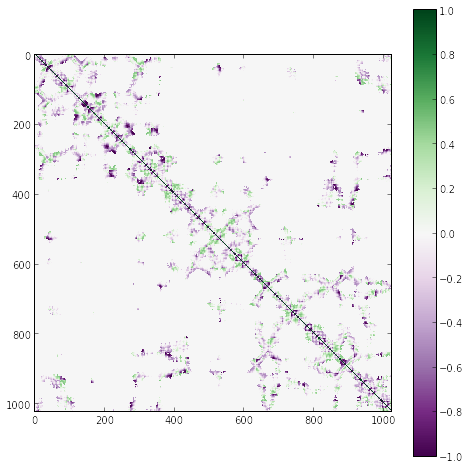
\includegraphics{/assets/normal_modes_files/normal_modes_14_0.png}

And then we diagonalize the Hessian matrix \(K\) above:

\begin{Shaded}
\begin{Highlighting}[]
\NormalTok{w,v }\OperatorTok{=}\NormalTok{ eig(K)}
\NormalTok{v }\OperatorTok{=}\NormalTok{ v[:,w.argsort()]}
\NormalTok{w }\OperatorTok{=}\NormalTok{ w[w.argsort()]}
\end{Highlighting}
\end{Shaded}

The sorted eigenvalues \(\lambda\) are plotted:

\begin{Shaded}
\begin{Highlighting}[]
\NormalTok{rcParams[}\StringTok{\textquotesingle{}figure.figsize\textquotesingle{}}\NormalTok{] }\OperatorTok{=} \DecValTok{8}\NormalTok{,}\DecValTok{4}
\NormalTok{plot(w, linewidth}\OperatorTok{=}\DecValTok{2}\NormalTok{)}
\NormalTok{xlabel(}\StringTok{\textquotesingle{}eigenvalue index\textquotesingle{}}\NormalTok{, fontsize}\OperatorTok{=}\DecValTok{14}\NormalTok{)}
\NormalTok{ylabel(}\StringTok{\textquotesingle{}$\textbackslash{}lambda$\textquotesingle{}}\NormalTok{, fontsize}\OperatorTok{=}\DecValTok{18}\NormalTok{)}
\NormalTok{grid()}
\end{Highlighting}
\end{Shaded}

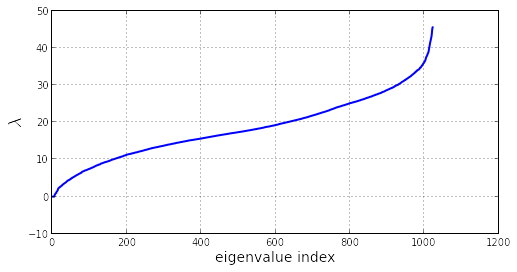
\includegraphics{/assets/normal_modes_files/normal_modes_18_0.png}

The first 6 eigenvalues are null (the 6 degrees of freedom of a rigid
body in a 3D space):

\begin{Shaded}
\begin{Highlighting}[]
\NormalTok{plot(w[:}\DecValTok{20}\NormalTok{], linewidth}\OperatorTok{=}\DecValTok{2}\NormalTok{)}
\NormalTok{xlabel(}\StringTok{\textquotesingle{}eigenvalue index\textquotesingle{}}\NormalTok{, fontsize}\OperatorTok{=}\DecValTok{14}\NormalTok{)}
\NormalTok{ylabel(}\StringTok{\textquotesingle{}$\textbackslash{}lambda$\textquotesingle{}}\NormalTok{, fontsize}\OperatorTok{=}\DecValTok{18}\NormalTok{)}
\NormalTok{grid()}
\end{Highlighting}
\end{Shaded}

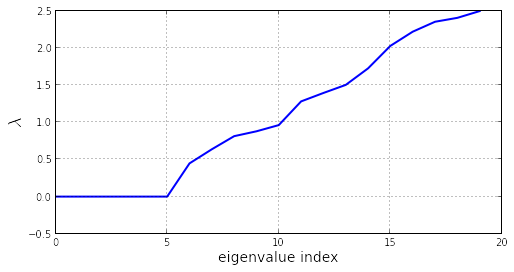
\includegraphics{/assets/normal_modes_files/normal_modes_20_0.png}

Then, we can compute the covariance and correlation matrix from the
inverse of the Hessian matrix \(K\):

\[K^{-1} = \sum_{i=7}^{3N} \frac{v_{i} \cdot v_{i}^{T}}{\lambda_{i}}\]

with \(N\) the number of considered atoms.

\begin{Shaded}
\begin{Highlighting}[]
\NormalTok{N }\OperatorTok{=}\NormalTok{ K.shape[}\DecValTok{0}\NormalTok{]}\OperatorTok{/}\DecValTok{3}
\NormalTok{hessian\_inv }\OperatorTok{=}\NormalTok{ zeros((}\DecValTok{3}\OperatorTok{*}\NormalTok{N,}\DecValTok{3}\OperatorTok{*}\NormalTok{N))}
\ControlFlowTok{for}\NormalTok{ i }\KeywordTok{in} \BuiltInTok{range}\NormalTok{(}\DecValTok{6}\NormalTok{,}\DecValTok{3}\OperatorTok{*}\NormalTok{N):}
\NormalTok{    hessian\_inv }\OperatorTok{+=}\NormalTok{ (dot(v[:,i][:,}\VariableTok{None}\NormalTok{],v[:,i][:,}\VariableTok{None}\NormalTok{].T)}\OperatorTok{/}\NormalTok{w[i])}
\end{Highlighting}
\end{Shaded}

The element of the covariance matrix is given by the trace of each
\(3 \times 3\) super element of \(K\). The diagonal of the covariance
matrix give the amplitude of the fluctuation for each considered atom of
the system.

\begin{Shaded}
\begin{Highlighting}[]
\NormalTok{rcParams[}\StringTok{\textquotesingle{}figure.figsize\textquotesingle{}}\NormalTok{] }\OperatorTok{=} \DecValTok{5}\NormalTok{,}\DecValTok{10}
\NormalTok{cov }\OperatorTok{=}\NormalTok{ zeros((N,N))}
\ControlFlowTok{for}\NormalTok{ i }\KeywordTok{in} \BuiltInTok{range}\NormalTok{(N):}
    \ControlFlowTok{for}\NormalTok{ j }\KeywordTok{in} \BuiltInTok{range}\NormalTok{(N):}
\NormalTok{        cov[i,j] }\OperatorTok{=}\NormalTok{ supertrace(hessian\_inv,i,j)}
\NormalTok{d }\OperatorTok{=}\NormalTok{ cov.diagonal()}
\NormalTok{subplot(}\DecValTok{211}\NormalTok{)}
\NormalTok{plot(d)}
\NormalTok{xlabel(}\StringTok{\textquotesingle{}sequence of considered atoms\textquotesingle{}}\NormalTok{, fontsize}\OperatorTok{=}\DecValTok{14}\NormalTok{)}
\NormalTok{ylabel(}\StringTok{\textquotesingle{}Amplitude of the fluctuation\textquotesingle{}}\NormalTok{, fontsize}\OperatorTok{=}\DecValTok{14}\NormalTok{)}
\NormalTok{grid()}
\NormalTok{corr }\OperatorTok{=}\NormalTok{ cov }\OperatorTok{/}\NormalTok{ sqrt(dot(d[}\VariableTok{None}\NormalTok{,:].T,d[}\VariableTok{None}\NormalTok{,:]))}
\NormalTok{subplot(}\DecValTok{212}\NormalTok{)}
\NormalTok{imshow(corr, vmax}\OperatorTok{=}\FloatTok{0.2}\NormalTok{)}
\NormalTok{title(}\StringTok{\textquotesingle{}Correlation matrix\textquotesingle{}}\NormalTok{, fontsize}\OperatorTok{=}\DecValTok{14}\NormalTok{)}
\NormalTok{tmp }\OperatorTok{=}\NormalTok{ colorbar()}
\end{Highlighting}
\end{Shaded}

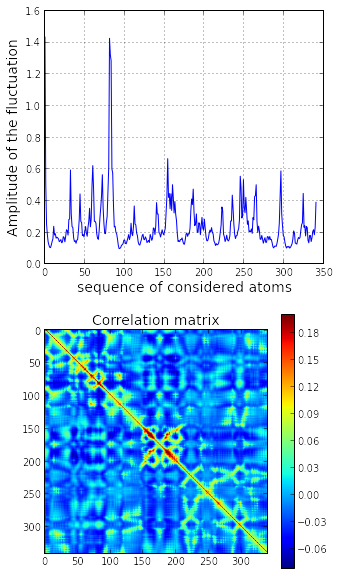
\includegraphics{/assets/normal_modes_files/normal_modes_24_0.png}

Now we can plot the first and the second mode on the structure. First I
align the protein on the three axes of inertia:

\begin{Shaded}
\begin{Highlighting}[]
\NormalTok{R}\OperatorTok{{-}=}\NormalTok{R.mean(axis}\OperatorTok{=}\DecValTok{0}\NormalTok{)}
\NormalTok{c,a }\OperatorTok{=}\NormalTok{ linalg.eig(dot(R.T,R))}
\NormalTok{R }\OperatorTok{=}\NormalTok{ dot(R,a)}
\end{Highlighting}
\end{Shaded}

And, here the plot for the first and second normal mode:

\begin{Shaded}
\begin{Highlighting}[]
\KeywordTok{def}\NormalTok{ plot\_mode(w, v, mode, cte }\OperatorTok{=} \DecValTok{50}\NormalTok{,doplot}\OperatorTok{=}\VariableTok{False}\NormalTok{):}
\NormalTok{    samples }\OperatorTok{=}\NormalTok{ R}
\NormalTok{    samples }\OperatorTok{{-}=}\NormalTok{ samples.mean(axis}\OperatorTok{=}\DecValTok{0}\NormalTok{)}
\NormalTok{    N,dim }\OperatorTok{=}\NormalTok{ samples.shape}
    \ControlFlowTok{if}\NormalTok{ doplot:}
\NormalTok{        fig }\OperatorTok{=}\NormalTok{ plt.figure(figsize}\OperatorTok{=}\NormalTok{(}\DecValTok{10}\NormalTok{,}\DecValTok{10}\NormalTok{))}
\NormalTok{        ax }\OperatorTok{=}\NormalTok{ fig.add\_subplot(}\DecValTok{111}\NormalTok{, projection}\OperatorTok{=}\StringTok{\textquotesingle{}3d\textquotesingle{}}\NormalTok{)}
\NormalTok{        ax.plot(samples[:,}\DecValTok{0}\NormalTok{], samples[:,}\DecValTok{1}\NormalTok{], samples[:,}\DecValTok{2}\NormalTok{], }\StringTok{\textquotesingle{}{-}\textquotesingle{}}\NormalTok{, markersize}\OperatorTok{=}\DecValTok{10}\NormalTok{, color}\OperatorTok{=}\StringTok{\textquotesingle{}green\textquotesingle{}}\NormalTok{, lw}\OperatorTok{=}\DecValTok{1}\NormalTok{)}
\NormalTok{        ax.scatter(samples[:,}\DecValTok{0}\NormalTok{], samples[:,}\DecValTok{1}\NormalTok{], samples[:,}\DecValTok{2}\NormalTok{], c}\OperatorTok{=}\BuiltInTok{range}\NormalTok{(samples.shape[}\DecValTok{0}\NormalTok{]), marker}\OperatorTok{=}\StringTok{\textquotesingle{}o\textquotesingle{}}\NormalTok{, s}\OperatorTok{=}\DecValTok{64}\NormalTok{)}
\NormalTok{    pc }\OperatorTok{=}\NormalTok{ v[:,mode].reshape(N,}\DecValTok{3}\NormalTok{)}
\NormalTok{    w }\OperatorTok{=}\NormalTok{ sqrt(w[mode])}
\NormalTok{    nstep}\OperatorTok{=}\DecValTok{100}
\NormalTok{    ts }\OperatorTok{=}\NormalTok{ linspace(}\OperatorTok{{-}}\NormalTok{w}\OperatorTok{*}\NormalTok{cte, w}\OperatorTok{*}\NormalTok{cte, nstep)}
\NormalTok{    interpolation}\OperatorTok{=}\NormalTok{zeros((nstep,N}\OperatorTok{*}\DecValTok{3}\NormalTok{))}
    \ControlFlowTok{for}\NormalTok{ j,t }\KeywordTok{in} \BuiltInTok{enumerate}\NormalTok{(ts):}
\NormalTok{        interpolation[j] }\OperatorTok{=}\NormalTok{ samples.flatten() }\OperatorTok{+}\NormalTok{ t}\OperatorTok{*}\NormalTok{pc.flatten()}
\NormalTok{    interpolation }\OperatorTok{=}\NormalTok{ interpolation.reshape(nstep,N,}\DecValTok{3}\NormalTok{)}
\NormalTok{    save(}\StringTok{\textquotesingle{}interpolation\textquotesingle{}}\NormalTok{, interpolation)}
    \ControlFlowTok{for}\NormalTok{ j,v }\KeywordTok{in} \BuiltInTok{enumerate}\NormalTok{(pc):}
\NormalTok{        x1,y1,z1 }\OperatorTok{=}\NormalTok{ samples[j]}
\NormalTok{        x2,y2,z2 }\OperatorTok{=}\NormalTok{ x1}\OperatorTok{+}\NormalTok{cte}\OperatorTok{*}\NormalTok{w}\OperatorTok{*}\NormalTok{v[}\DecValTok{0}\NormalTok{], y1}\OperatorTok{+}\NormalTok{cte}\OperatorTok{*}\NormalTok{w}\OperatorTok{*}\NormalTok{v[}\DecValTok{1}\NormalTok{], z1}\OperatorTok{+}\NormalTok{cte}\OperatorTok{*}\NormalTok{w}\OperatorTok{*}\NormalTok{v[}\DecValTok{2}\NormalTok{]}
        \ControlFlowTok{if}\NormalTok{ doplot:}
\NormalTok{            ax.plot([x1,x2], [y1,y2], [z1,z2], color}\OperatorTok{=}\StringTok{\textquotesingle{}red\textquotesingle{}}\NormalTok{, alpha}\OperatorTok{=}\FloatTok{0.8}\NormalTok{, lw}\OperatorTok{=}\DecValTok{2}\NormalTok{)}
    \ControlFlowTok{return}\NormalTok{ pc}


\NormalTok{tmp }\OperatorTok{=}\NormalTok{ plot\_mode(w, v, }\DecValTok{6}\NormalTok{, doplot}\OperatorTok{=}\VariableTok{True}\NormalTok{)}
\NormalTok{title(}\StringTok{\textquotesingle{}Normal mode \#1\textquotesingle{}}\NormalTok{)}
\NormalTok{tmp }\OperatorTok{=}\NormalTok{ plot\_mode(w, v, }\DecValTok{7}\NormalTok{, doplot}\OperatorTok{=}\VariableTok{True}\NormalTok{)}
\NormalTok{title(}\StringTok{\textquotesingle{}Normal mode \#2\textquotesingle{}}\NormalTok{)}
\end{Highlighting}
\end{Shaded}

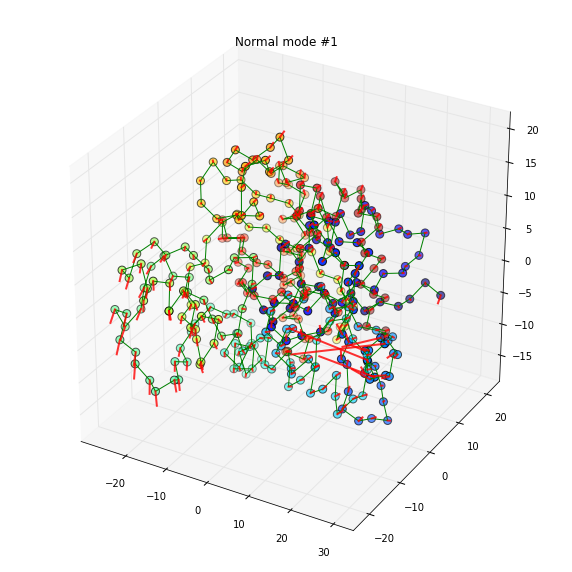
\includegraphics{/assets/normal_modes_files/normal_modes_29_0.png}

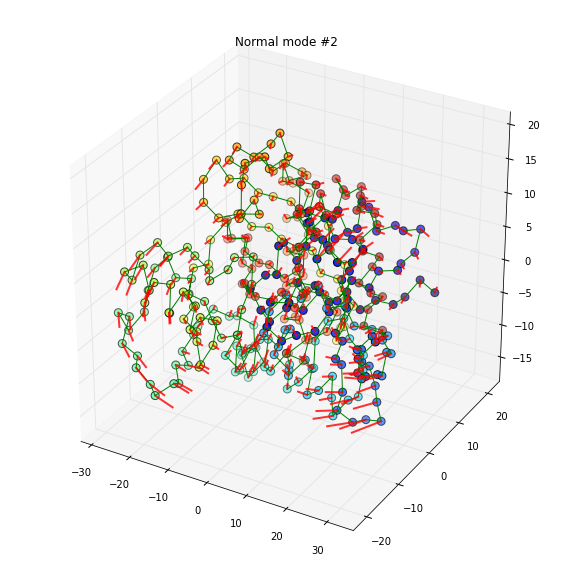
\includegraphics{/assets/normal_modes_files/normal_modes_29_1.png}

The first mode is predominated by the movement of a losely connected
loop. The 2nd mode arises a more correlated global motion.

Below an interpolation along the second mode:

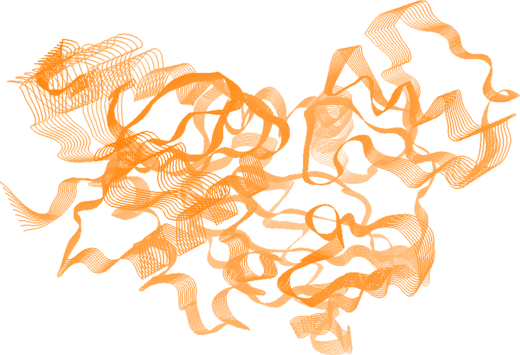
\includegraphics{/assets/normal_modes_files/vana_second_mode.png}

{If you want to ask me a question or leave me a message add @bougui505
in your comment.}

\href{http://stackexchange.com/users/1853608/bougui}{\includegraphics[width=2.16667in,height=0.60417in]{http://stackexchange.com/users/flair/1853608.png}}

\hypertarget{bloggb}{%
\subsection{bloggb}\label{bloggb}}

\begin{itemize}
\tightlist
\item
  bloggb
\item
  \href{mailto:}{}
\end{itemize}

\begin{itemize}
\tightlist
\item
  \href{https://github.com/bougui505}{{ } {bougui505}}
\item
  \href{https://twitter.com/bougui505}{{ } {bougui505}}
\end{itemize}

Blog of Guillaume Bouvier

\href{http://creativecommons.org/licenses/by-sa/4.0/}{\includegraphics{https://i.creativecommons.org/l/by-sa/4.0/88x31.png}}\\
This work by \href{http://izar.crabdance.com/}{Guillaume Bouvier} is
licensed under a
\href{http://creativecommons.org/licenses/by-sa/4.0/}{Creative Commons
Attribution-ShareAlike 4.0 International License}.

\end{document}
